{\centering
\noindent{\Large \textbf{Word Meaning, in Computational Linguistics and Beyond}}\\  \vspace*{-0.1cm} \leavevmode\newline
{\normalsize \textbf{Katrin Erk}}\\
{\normalsize {University of Texas at Austin, USA}}\\


\begin{figure}[h!]
  \centering
      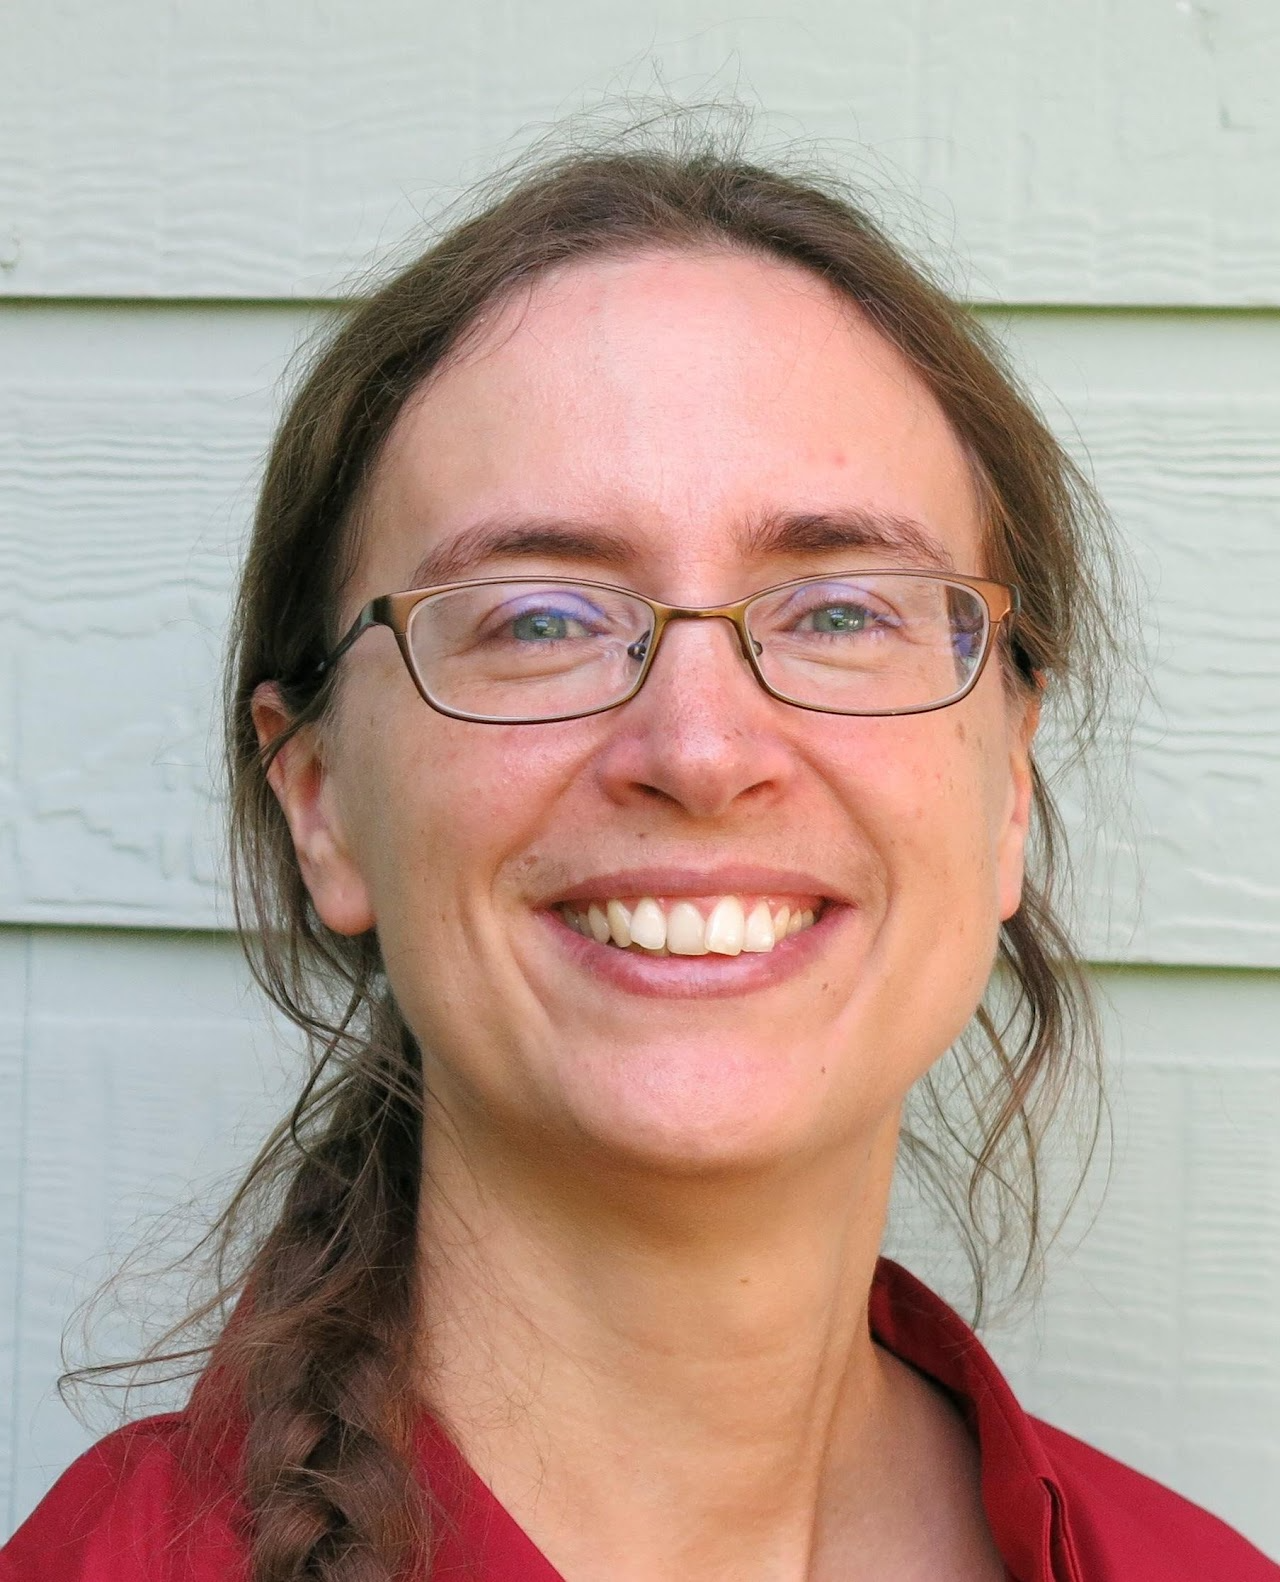
\includegraphics[width=0.15\linewidth]{examples/handbook_coling25/invited_talks/katrin_erk_invited_2.png}
\end{figure}

 {\normalsize \textbf{Wednesday, Jan 22, 2025} -
 Room: \textbf{Conference Hall A} -
 Time: \textbf{16:00-17:00}\\\leavevmode\newline
 }
}

{\textbf{Abstract:}}
What kinds of things are word meanings, and how can we model them computationally? In the time of distributional models, the study of polysemy structure always seemed just out of reach. Now, recent language models provide exhilarating new prospects for studying lexical meaning: Looking at embeddings, we can finally see usage groups, both similar to and intriguingly different from dictionary senses, especially in the cultural traces or “story traces” that they show. With prompting, we can get at more complex structures of meaning, like properties of frames and narratives. But there is so much to be figured out first. We have many promising techniques, but we don’t yet have reliable best practices and tools for analyzing language models for lexical meaning. It is also still difficult to distinguish the signal from the noise: When the picture that language models show us of word meaning diverges from how we humans organize dictionaries, then which parts are important facets of meaning that we have overlooked, and which parts are just peculiarities of the computational system? To make progress here, we also need to further develop our theories of the lexicon.\\

{\textbf{Bio:}}
Katrin Erk is a Professor of Linguistics and Computer Science at the University of Texas at Austin. She earned her Ph.D. from Saarland University in Germany in 2002, focusing on tree description languages and ellipsis. Her research expertise lies in computational linguistics, particularly in semantics. She specializes in developing distributed, flexible approaches to describing word meaning and integrating them with representations at the sentence or discourse level. Her work includes studying flexible representations of word meaning constrained by context and exploring frameworks that draw inferences based on sentence structure and word meanings. She also investigates narrative schemas and their influence on word meaning and inference. In October 2024, it was announced that she will join the University of Massachusetts Amherst in September 2025, holding a joint position in the Department of Linguistics and the Manning College of Information and Computer Sciences. Throughout her career, she has received several awards and honors, including a CSLI Fellowship at Stanford in 2017 and a Google Faculty Research Award in 2018.\\

\clearpage